All code is found at https://github.com/Oscarlsson/RL-competition

Improvements using tiebreaker?!

When testing our agent on very different environments, from simple board games to context bandit problems. We observe that even very general approaches to improving performance against a large class of environments, might hurt the performance against other environments. We addressed large state space environments, where the state is altered gradually and good actions are good over a range of similar states, and introduced a tie breaker that tries to make informed decisions when faced with a lack of statistical data. This replaced a simple "first best" choice, which turned out to actually be a better decision in some cases. 

Running the agent with varying step sizes $\alpha$ we observed bad results on all values but $\alpha=1$. Similarly, for most $\lambda$ values...KOLLA HÄR!!


Sweep $\lambda$
\begin{figure}[h]
    \centering
    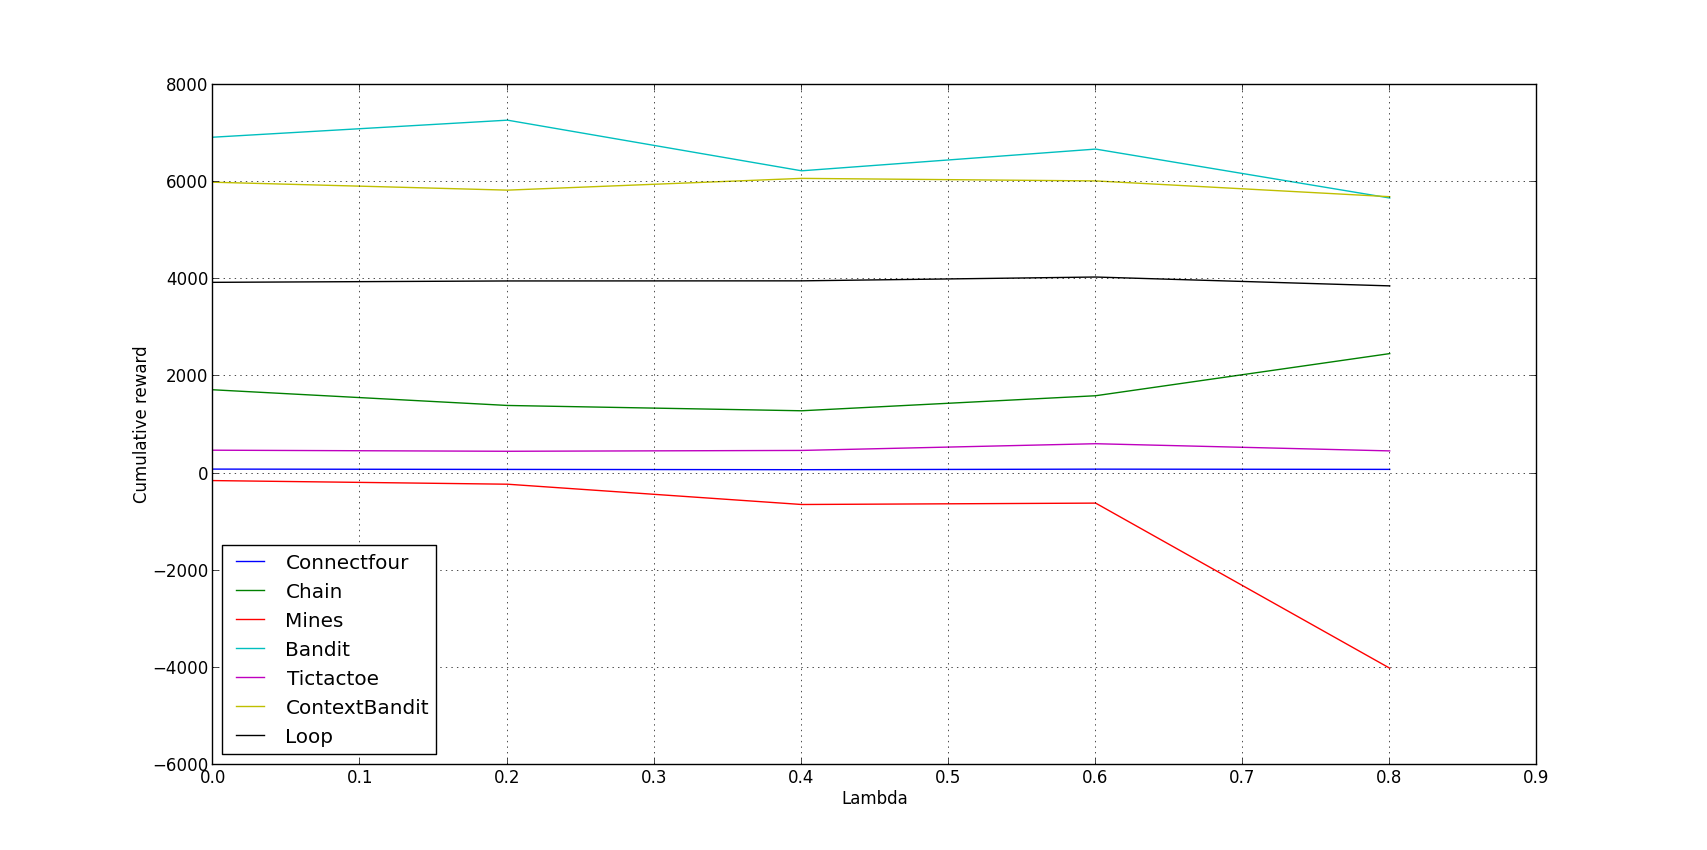
\includegraphics[width=0.5\textwidth]{../data/lambdasweepplot.png}
    \caption{Awesome Image}
    \label{fig:awesome_image}
\end{figure}


Figure~\ref{fig:cumreward} shows how the agents average performance over 50 runs in a 100 episode experiment against all environments with parameters set to $\lambda = 0.2$ and $\alpha = 1$

\begin{figure}[h!]
    \centering
    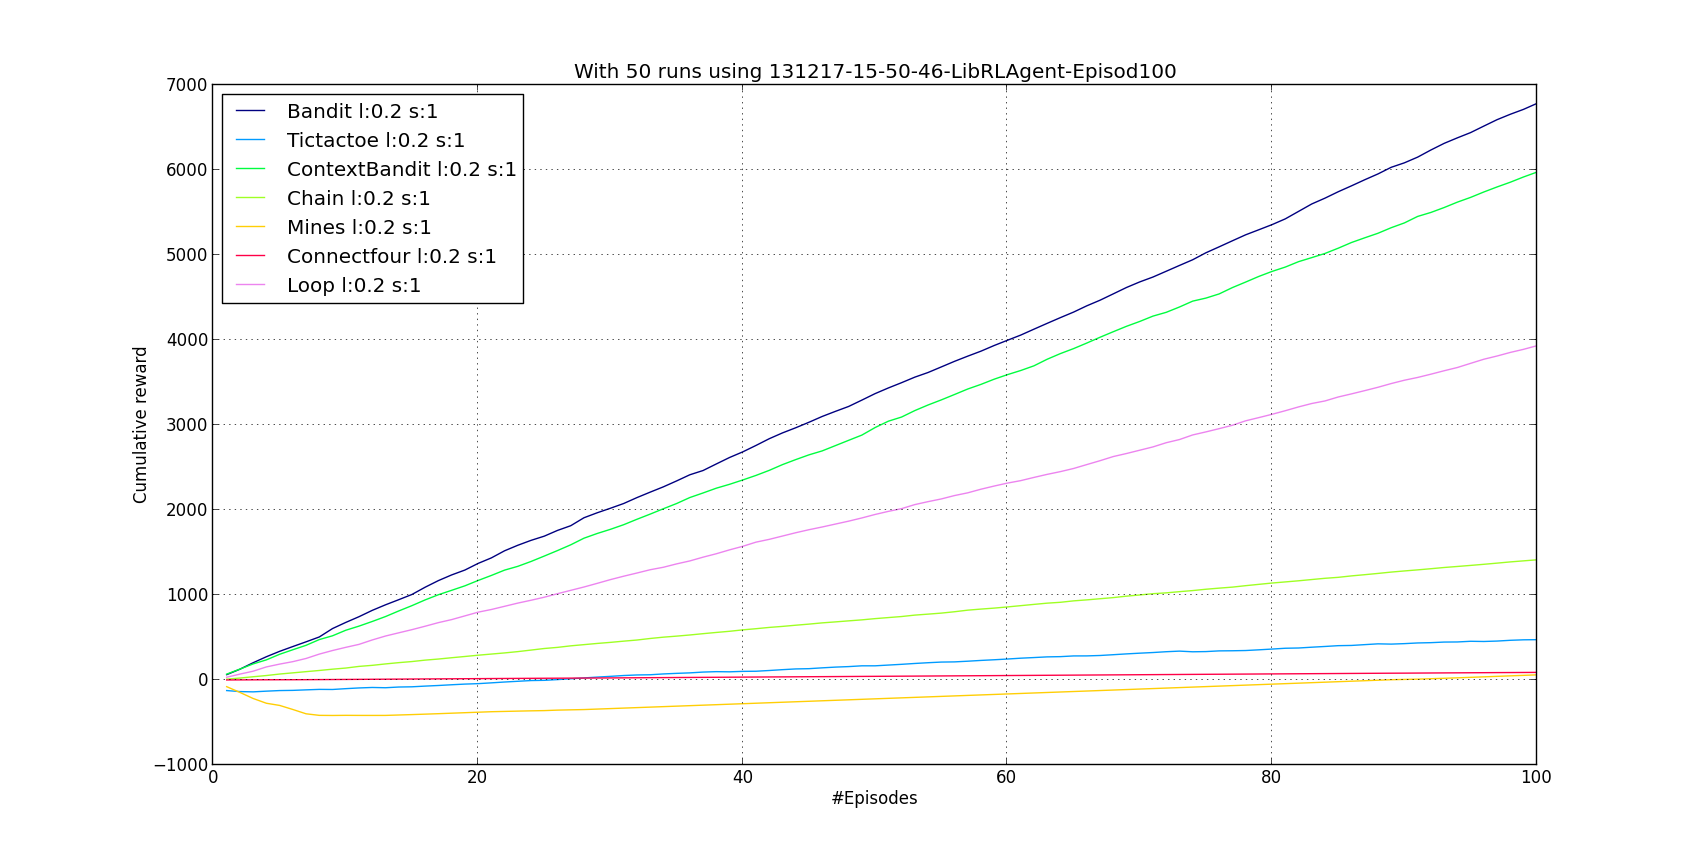
\includegraphics[width=0.5\textwidth]{../data/100episodes_50runs.png}
    \caption{Agents cumulative reward averaged over 50 runs}
    \label{fig:cumreward}
\end{figure}

Sweep $\lambda$
\begin{figure}[h]
    \centering
    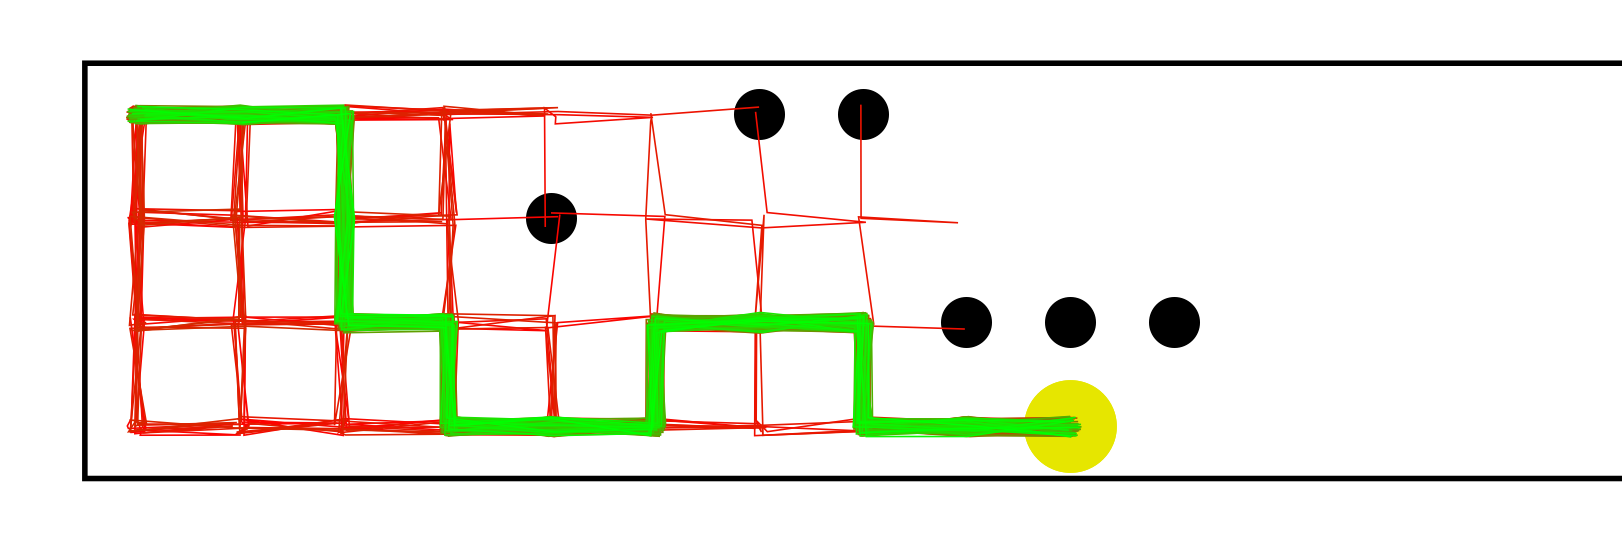
\includegraphics[width=0.5\textwidth]{../data/minPlot.png}
    \caption{Example of how the agent learns a short path from start to goal (yellow). The agent traverse the world 100 times, early attempts are coloured red, later green. Hitting a mine (black) costs a penalty. Every  }
    \label{fig:awesome_image}
\end{figure}

The yellow line indicates the performance on the mines environment and the learning phase of the agent is clear after around 10 episodes. Connect four, red in Fig~\ref{fig:cumreward}, has a much lower maximum reward than the other environments hence it is closer to zero but still increasing.
